\label{sec:segmentation}

Segmentation is another subtask in the image domain.
The target here is to obtain a mask of an object or objects in an image.
It is related to the classical classification problem, but instead of predicting the class for a whole image, the class is here predicted for each pixel individually.
Segmentation can be further divided into semantic segmentation \cite{semantic_segmentation} and instance segmentation \cite{mask_rcnn}.
In semantic segmentation the type of an object in general is predicted for example cat or dog.
In instance segmentation further the instance of an object is predicted so, e.g. when two cats are present two separate masks would be predicted.
Figure \ref{fig:instance_vs_semantic} illustrates the two different types of segmentation.

\begin{figure}
\begin{center}
    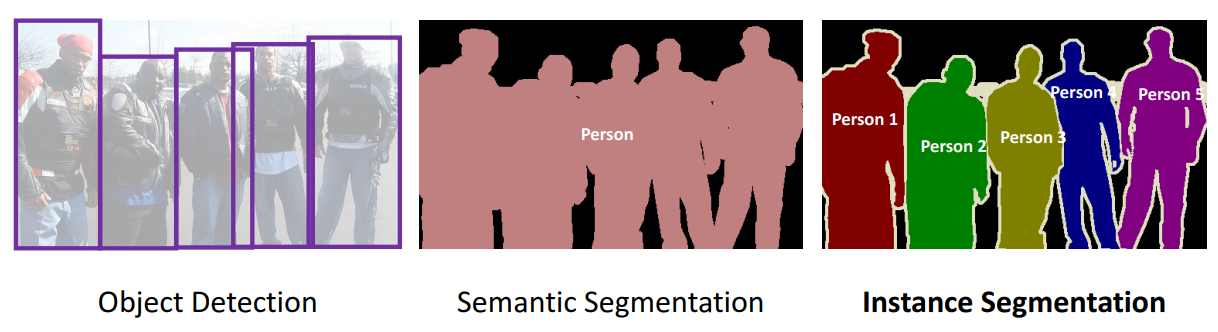
\includegraphics[width=16cm]{imgs/instance_vs_semantic_seg.png}
    \caption{The difference between object detection, semantic segmentation and instance segmentation. In object detection the instance with a rough estimate (bounding box) is predicted, in semantic segmentation a segmentation mask for an object is predicted without considering the underlying instance and in instance segmentation the instance as well as a segmentation mask for an object is predicted. \cite{instance_vs_semantic_fig}}
    \label{fig:instance_vs_semantic}
\end{center}
\end{figure}

\section{MobileNetV2-UNet}
\label{sec:mobilenetv2_unet}

For the segmentation of the circuits \ac{MUnet} \cite{mobile_unet} is used.
This network is build upon the principles of the famous U-Net proposed by Ronneberger et al. \cite{unet}.
The classical U-Net architecture consists of two main components: an encoder and a decoder.
The encoder is a classical \ac{CNN} which learns the features of the provided data.
It uses convolutional layers and max pooling layers to downsample the feature map size.
The decoder does the inverse, here the feature maps are convolved and then upsampled.
Which made the U-Net unique at the proposed time is that to enhance the segmentation results, additionally after a feature map was upsampled it gets concatenated with a feature map from the backbone which has the same resolution.
It should be noted that this approach was probably picked up by the \ac{YOLOv4} developers and reused in their architecture as has been shown in section \ref{sec:yolo}.

\ac{MUnet} is a combination of the MobileNetV2 \cite{mnetv2} which is used as the backbone and a decoder which is adapted to the backbone.
In the following section the architecture of the \ac{MUnet} is explained.

\subsubsection{MobileNetV2-UNet backbone}

MobileNetV2 is the backbone of the \ac{MUnet} and can be decomposed into two main components:

\begin{itemize}
    \item depthwise separable convolutions
    \item inverted residual blocks
\end{itemize}

Depthwise separable convolutions were already used in the first MobileNet and are a way to factorize a standard convolution into a depthwise convolution and a $1\times1$ convolution.
Essentially this means that a classical convolution is split into two layers, in the depthwise convolutional layer first a convolution is applied on each channel separately, i.e. given an input $I \in \R^{H \times W \times C}$ and $C$ kernels $K^{h \times w \times 1}$ each channel $C_i$ is convolved with a corresponding kernel $K_i$.
Afterwards, to build up features lightweight $1 \times 1$ convolutions are used.
This method has shown to perform almost on par with a classical convolution, but reduces the amount of computation by a factor of eight \cite{mnetv1}.
Hence, this method is perfectly suited for resource constrained environments such as mobile phones.

The inverted residual layer is a novel layer in MobileNetV2.
The idea is to first project the input feature maps into a lower dimensional subspace by using a $1 \times 1$ convolution with ReLU6 non-linearity, the resulting feature maps are then expanded inside the block by a following depthwise separable convolution.
Afterwards, the output is again convolved with $1 \times 1$ convolution.
Further, the inverted residual has a residual connection where the input is added to the output of the last linear $1 \times 1$ convolution.
The whole inverted residual block can be seen in figure \ref{fig:inverted_residual} it also shows that the input gets expanded inside the inverted residual block.
The expansion factor $t \in \N$ defines how much the input is expanded inside the inverted residual block.
The expansion can be seen in table \ref{tab:invres_expansion}.

\begin{table} %[H]
\begin{center}

\begin{tabular}{l|l|l}
\textbf{Input} & \textbf{Operator} & \textbf{Output}\\
\hline
$h \times w \times k$ & $1 \times 1$ conv2d, BatchNorm, ReLU6 & $h \times w \times (tk)$\\
$h \times w \times (tk)$ & $3 \times 3$ dwise s=s, BatchNorm, ReLU6 & $\frac{h}{s} \times \frac{w}{s} \times (tk)$ \\
$\frac{h}{s} \times \frac{w}{s} \times (tk)$ & $1 \times 1$ conv2d, BatchNorm & $\frac{h}{s} \times \frac{w}{s} \times k'$
\end{tabular}

\caption{An inverted residual block transforming from $k$ to $k'$ channels, with stride $s$ and expansion factor $t$.}
\label{tab:invres_expansion}
\end{center}
\end{table}

\begin{figure}
\begin{center}
    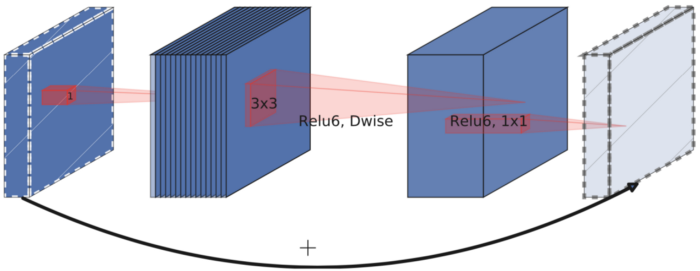
\includegraphics[width=13cm]{imgs/inverted_residual.png}
    \caption{The inverted residual block. A $1 \times 1$ convolution with non-linear activation followed by a depthwise separable convolution and a linear $1 \times 1$ convolution with residual connection to the input. The residual connection is here additive, i.e. the input gets added to the output of the linear $1 \times 1$ convolution.}
    \label{fig:inverted_residual}
\end{center}
\end{figure}

% The development of this layer was guided by the important factors that feature maps are able to be encoded in low-dimensional subspaces and that the use of \ac{ReLU} can result in information loss if input features are not embedded in a low-dimensional subspace \cite{mnetv2}.
% So the idea behind the layers is when first the input features get embedded into a low-dimensional subspace

The whole MobileNetV2 architecture is given in table \ref{tab:mobilenetv2_architecture}.

\begin{table} %[H]
\begin{center}

\begin{tabular}{l|l|l|l|l|l|l|l}
\textbf{Blocks} & \textbf{Operation} & \textbf{t} & \textbf{k} & \textbf{n} & \textbf{s} & \textbf{Output (h, w, c)}\\
\hline
Input           & -             & - & - & - & - & (448, 448, 3) \\
                & Conv+BN+ReLU6 & - & 3 & 1 & 2 & (224, 244, 32) \\
$Skip_{1}$      & InvRes        & 1 & - & 1 & 1 & (224, 224, 16)\\
$Skip_{2}$      & InvRes        & 6 & - & 2 & 2 & (112, 112, 24) \\
$Skip_{3}$      & InvRes        & 6 & - & 3 & 2 & (56, 56, 32) \\
                & InvRes        & 6 & - & 4 & 2 & (28, 28, 64) \\
$Skip_{4}$      & InvRes        & 6 & - & 3 & 1 & (28, 28, 96) \\
                & InvRes        & 6 & - & 3 & 2 & (14, 14, 160) \\
                & InvRes        & 6 & - & 1 & 1 & (14, 14, 320) \\
$Skip_{5}$      & Conv+BN+ReLU6 & - & 1 & - & - & (14, 14, 1280) \\
\end{tabular}

\caption{MobileNetV2 backbone used in \ac{MUnet} Blocks marked as $Skip_*$ are outputs from the network which are used in the decoder. The parameters above define the configuration of the respective block, $t$ is the expansion factor inside an inverted residual block as defined in \ref{tab:invres_expansion}, $k$ is the kernel size for the two standard convolutions used in the backbone, $n$ defines how often that particular block is repeated and $s$ is the stride of a block. Note that if $s = 2$ only the first block has this stride, the others have $s = 1$.}
\label{tab:mobilenetv2_architecture}
\end{center}
\end{table}

\subsubsection{MobileNetV2-UNet decoder}

The decoder of \ac{MUnet} is build by the principles of U-Net\cite{unet}.
Feature map upsampling is done using transposed convolutions.
After a feature map has been upsampled it is concatenated with a skip connection from the backbone with the same spatial dimension.
Concatenation is performed along the channel axis.
To unify the novel concatenated feature map it is passed to a inverted residual block.
This step is repeated until no skip connections from the backbone are left.
The last step in the decoder is composed of a bilinear upsampling layer, which is used to produce a prediction which has the same size as the input image.
This has to be done because the backbone directly downsamples the image size in the first layer and hence there is no feature map with the same spatial dimensions as the input image.
The architecture of the backbone can be found in table \ref{tab:mobilenetv2_decoder}.

\begin{table} %[H]
\begin{center}

\begin{tabular}{l|l|l|l|l|l|l|l}
\textbf{Block} & \textbf{Inputs} & \textbf{Operation} & \textbf{t} & \textbf{k} & \textbf{s} & \textbf{Output (h, w, c)}\\
\hline
$Up1$     & $Skip_5$        & ConvTranspose & - & 4 & 2 & (28, 28, 96) \\
$InvRes1$ & $Skip_4 + Up1$  & InvRes        & 6 & - & 1 & (28, 28, 96) \\
$Up2$     & $InvRes1$       & ConvTranspose & - & 4 & 2 & (56, 56, 32) \\
$InvRes2$ & $Skip_3 + Up2$  & InvRes        & 6 & - & 1 & (56, 56, 32) \\
$Up3$     & $InvRes2$       & ConvTranspose & - & 4 & 2 & (112, 112, 24) \\
$InvRes3$ & $Skip_2 + Up3$  & InvRes        & 6 & - & 1 & (112, 112, 24) \\
$Up4$     & $InvRes3$       & ConvTranspose & - & 4 & 2 & (224, 224, 16) \\
$InvRes4$ & $Skip_1 + Up4$  & InvRes        & 6 & - & 1 & (224, 224, 2) \\
$Up5$     & $InvRes4$       & UpBillinear   & - & - & 2 & (448, 448, 2) \\
\end{tabular}

\caption{\ac{MUnet} decoder. The decoder uses transpose convolutions to upsample the input (ConvTranspose) and as the backbone, inverted residuals to process the upsampled input together with the skip connection. The '+' indicates a concatenation along the channel axis. Since the first block in the backbone directly downsamples the input there is no skip connection with the size of the input. Therefore the last layer of the decoder is a upsampling layer, which uses a bilinear upsampling method to increase the size of the prediction to the size of the input. As with the backbone $t$ indicates the expansion size of the inverted residual block, $k$ indicates the used kernel size and $s$ indicates the used stride.}
\label{tab:mobilenetv2_decoder}
\end{center}
\end{table}
